\documentclass[lecture.tex]{subfiles}

\begin{document}

\exercice{}
%\video{https://youtu.be/blablabla}
\enonce{rdm-0059}{Efforts internes}

Une poutre de longueur $3L$, appuyée en $A$ (rotule) et $B$ (appui ponctuel), est soumis à un effort ponctuel en $B$ et un effort linéique $f$ selon l'axe $Y$ après le point $C$, comme illustré sur le schéma ci-dessous

\begin{figure}[h!]
  \centering
  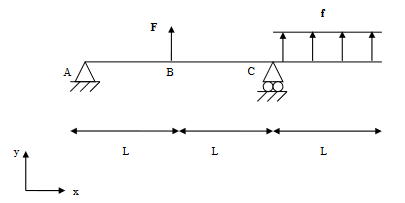
\includegraphics[scale=0.8]{fig1-rdm-0059.png}
\end{figure}

On notera les efforts appliqués de la façon suivante :
\begin{itemize}
  \item[$\bullet$] $\vec{F}_B = F \vec{y}$ avec  $F>0$
  \item[$\bullet$] $\vec{f} = f \vec{y}$ avec $f>0$
\end{itemize}

Les efforts de liaison seront quant à eux notés :
\begin{itemize}
  \item[$\bullet$] en $A$, $\vec{F}_A = F_{xA} \vec{x} + F_{yA} \vec{y}$
  \item[$\bullet$] en $C$, $\vec{F}_C = F_{xC} \vec{x} + F_{yC} \vec{y}$
\end{itemize}

\bigskip

\begin{enumerate}
  \item Déterminer le degré d'hyperstaticité du système.

  \item A l'aide d'une étude statique, déterminer les efforts de liaisons en $A$ et en $C$

  \item Déterminer les efforts internes dans la poutre pour $0 < x < L$.

  \item Déterminer les efforts internes dans la poutre pour $L < x < 2L$.

  \item Déterminer les efforts internes dans la poutre pour $2L < x < 3L$.

  \item Vérifier que quel que soit $x$ on a bien $\displaystyle T=-\frac{d M}{d x}$.

  \item Tracer les trois diagrammes des efforts internes de la poutre.

\end{enumerate}

\finenonce{rdm-0059}
\finexercice


\end{document}
